% SHILATE — Bachelor's Thesis Presentation
% 7-minute academic slide deck — LaTeX Beamer
% Compile: pdflatex presentation.tex

\documentclass[aspectratio=169]{beamer}

\usetheme{CambridgeUS}
\usecolortheme{beaver}

\usepackage[T1]{fontenc}
\usepackage[english]{babel}
\usepackage{microtype}
\usepackage{graphicx}
\usepackage{booktabs}
\usepackage{amsmath}
\usepackage{tikz}
\usetikzlibrary{positioning,arrows.meta,shapes.geometric,fit,backgrounds}

% ─── Palette tweaks ──────────────────────────────────────────────────────────
\definecolor{upt-navy}{RGB}{0,56,101}
\definecolor{upt-red}{RGB}{184,14,27}
\definecolor{upt-gray}{RGB}{88,88,88}

\setbeamercolor{title}{fg=white,bg=upt-navy}
\setbeamercolor{frametitle}{fg=white,bg=upt-navy}
\setbeamercolor{section in head/foot}{fg=white,bg=upt-navy}
\setbeamercolor{subsection in head/foot}{fg=white,bg=upt-red}
\setbeamercolor{author in head/foot}{fg=white,bg=upt-navy}
\setbeamercolor{date in head/foot}{fg=white,bg=upt-red}
\setbeamercolor{title in head/foot}{fg=white,bg=upt-navy}
\setbeamercolor{item}{fg=upt-red}
\setbeamercolor{structure}{fg=upt-navy}
\setbeamercolor{block title}{bg=upt-navy,fg=white}
\setbeamercolor{block body}{bg=upt-navy!8}
\setbeamercolor{alerted text}{fg=upt-red}

\setbeamerfont{title}{size=\large,series=\bfseries}
\setbeamerfont{frametitle}{size=\normalsize,series=\bfseries}

% ─── Metadata ────────────────────────────────────────────────────────────────
\title[SHILATE]{SHILATE\\[4pt]
  \small Software Hardware In Loop\\Automotive Testing Environment}
\author[Tudor-Ciprian Tămaș]{Tudor-Ciprian Tămaș\\[2pt]
  {\footnotesize Supervisor: Sl.~Dr.~Ing.~Valentin Mărănescu}}
\institute[UPT]{
  \textit{Electronics, Telecommunications and Information Technology}\\
  Politehnica University of Timișoara}
\date{July 2026}

% ─── Helpers ─────────────────────────────────────────────────────────────────
\newcommand{\mqttarrow}[0]{\textcolor{upt-red}{\(\boldsymbol{\leftrightarrow}\)}\,MQTT\,\textcolor{upt-red}{\(\boldsymbol{\leftrightarrow}\)}}

% ─── Suppress navigation symbols ─────────────────────────────────────────────
\setbeamertemplate{navigation symbols}{}

% ─── Progress bar in footline ────────────────────────────────────────────────
\setbeamertemplate{footline}{%
  \leavevmode%
  \hbox{%
    \begin{beamercolorbox}[wd=.45\paperwidth,ht=2.5ex,dp=1ex,left,leftskip=1em]{author in head/foot}%
      \usebeamerfont{author in head/foot}\insertshortauthor
    \end{beamercolorbox}%
    \begin{beamercolorbox}[wd=.45\paperwidth,ht=2.5ex,dp=1ex,center]{title in head/foot}%
      \usebeamerfont{title in head/foot}\insertshorttitle
    \end{beamercolorbox}%
    \begin{beamercolorbox}[wd=.10\paperwidth,ht=2.5ex,dp=1ex,right,rightskip=1em]{date in head/foot}%
      \usebeamerfont{date in head/foot}
      \insertframenumber{}/\inserttotalframenumber
    \end{beamercolorbox}}%
  \vskip0pt%
}

% =============================================================================
\begin{document}
% =============================================================================

% ─── SLIDE 1 — Title ─────────────────────────────────────────────────────────
\begin{frame}
  \vspace{0.5em}
  \begin{columns}[c]
    \column{0.72\textwidth}
      \titlepage
    \column{0.28\textwidth}
      \centering
      
\includegraphics[width=0.88\linewidth]{images/logo.png}
  \end{columns}
\end{frame}

% ─── SLIDE 2 — Motivation ────────────────────────────────────────────────────
\begin{frame}{Motivation}
  \begin{columns}[T]
    \column{0.52\textwidth}
      \textbf{The Industry Shift}
      \begin{itemize}\setlength\itemsep{5pt}
        \item Vehicles are becoming \alert{software-defined} — behaviour updated over-the-air
        \item Reinforcement learning (RL) is maturing as a practical control tool
        \item But no open-source pipeline bridges \textbf{RL training} and \textbf{SDV deployment}
      \end{itemize}
      \vspace{0.8em}
      \textbf{Four Open Challenges}
      \begin{enumerate}\setlength\itemsep{3pt}
        \item Simulation $\leftrightarrow$ middleware protocol coupling
        \item Standardised signal representation (VSS)
        \item Operational safety monitoring of learned policies
        \item Reproducible, one-click training workflow
      \end{enumerate}

    \column{0.45\textwidth}
      \begin{block}{Goal}
        Build an \textbf{end-to-end, open-source} pipeline that:
        \begin{itemize}\setlength\itemsep{4pt}
          \item Trains a deep RL agent in a Unity physics sim
          \item Deploys the policy onto a real Eclipse Leda SDV stack
          \item Uses the \textbf{same MQTT / VSS layer} from training to hardware
        \end{itemize}
      \end{block}
  \end{columns}
\end{frame}

% ─── SLIDE 3 — System Architecture ──────────────────────────────────────────
\begin{frame}{System Architecture — Three Loosely Coupled Tiers}
  \begin{columns}[T]
    \column{0.46\textwidth}
      \begin{tikzpicture}[
          box/.style={
            draw=upt-navy, fill=upt-navy!8, rounded corners=4pt,
            text width=4.2cm, minimum height=1.05cm,
            align=center, font=\small},
          mqttbox/.style={
            draw=upt-red, fill=upt-red!10, rounded corners=3pt,
            text width=4.2cm, minimum height=0.55cm,
            align=center, font=\footnotesize\itshape},
          arr/.style={-{Stealth[length=5pt]}, upt-red, line width=1.1pt}
        ]
        \node[box] (unity) {%
          \textbf{Tier~1: Unity Simulation}\\[-1pt]
          {\footnotesize Vehicle physics · LiDAR · Training Controller}};
        \node[mqttbox, below=0.18cm of unity] (mqtt1)
          {Mosquitto MQTT broker};
        \node[box, below=0.18cm of mqtt1] (python) {%
          \textbf{Tier~2: Python PPO}\\[-1pt]
          {\footnotesize Stable-Baselines3 · Gymnasium env}};
        \node[mqttbox, below=0.18cm of python] (mqtt2)
          {Mosquitto MQTT broker};
        \node[box, below=0.18cm of mqtt2] (leda) {%
          \textbf{Tier~3: Eclipse Leda SDV}\\[-1pt]
          {\footnotesize Kuksa · feeder · Velocitas · RPi~4}};
        \draw[arr] (unity.south) -- (mqtt1.north);
        \draw[arr] (mqtt1.south) -- (python.north);
        \draw[arr] (python.south) -- (mqtt2.north);
        \draw[arr] (mqtt2.south) -- (leda.north);
      \end{tikzpicture}

    \column{0.52\textwidth}
      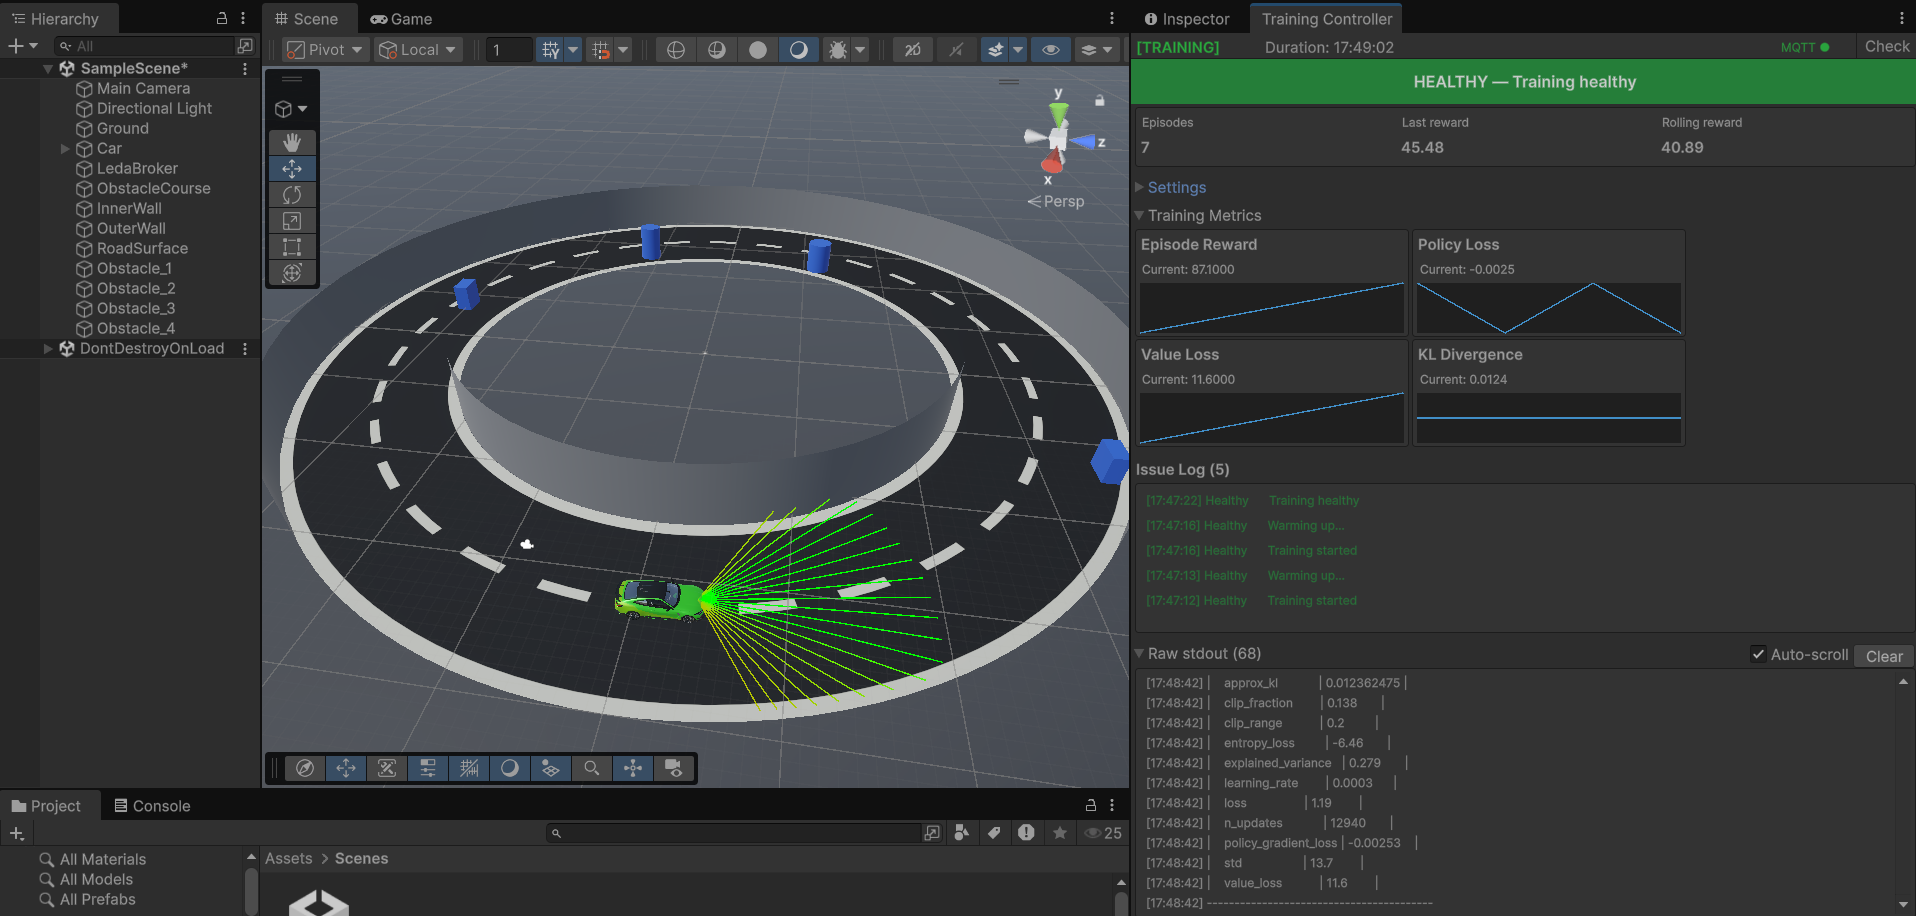
\includegraphics[width=\linewidth]{images/enviroment_overview.png}
      {\centering\footnotesize\textcolor{upt-gray}{Simulation environment overview}\par}

      \vspace{0.5em}
      \begin{itemize}\setlength\itemsep{4pt}
        \item All inter-tier traffic flows through \alert{MQTT topic prefix \texttt{env0/}}
        \item No direct function calls across tiers — fully decoupled
        \item Same topic namespace in training \textbf{and} on hardware
      \end{itemize}
  \end{columns}
\end{frame}

% ─── SLIDE 4 — Unity Simulation ──────────────────────────────────────────────
\begin{frame}{Unity Simulation Component}
  \begin{columns}[T]
    \column{0.42\textwidth}
      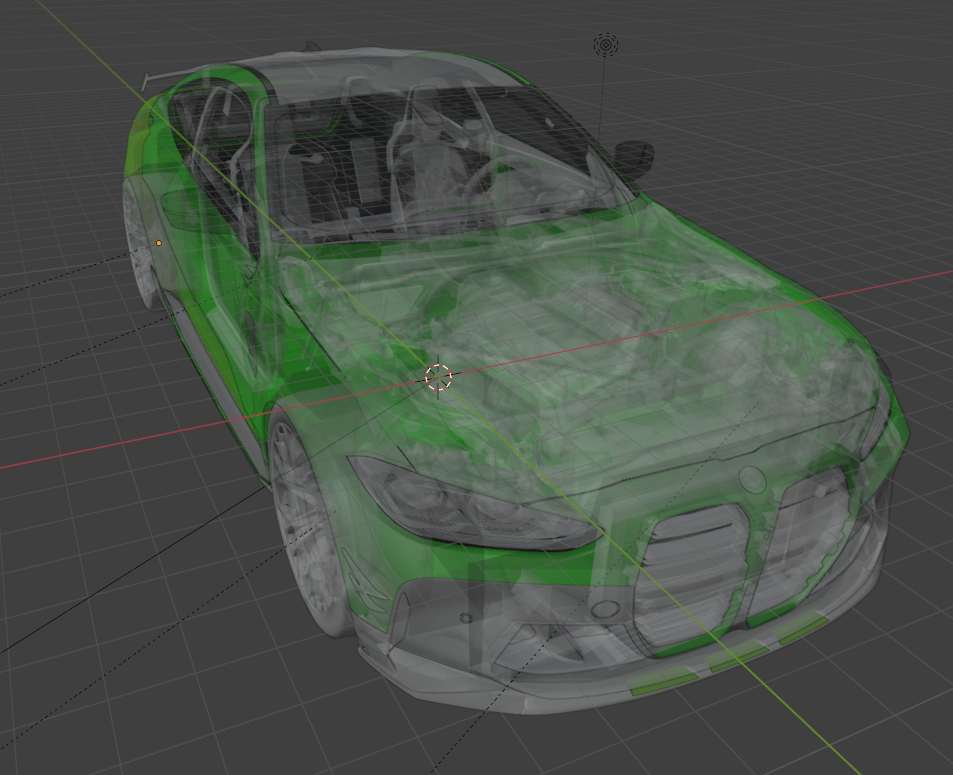
\includegraphics[width=\linewidth]{images/car_model_transparent.png}
      {\centering\footnotesize\textcolor{upt-gray}{Rear-wheel-drive vehicle model}\par}

    \column{0.56\textwidth}
      \textbf{Vehicle \& Sensor}
      \begin{itemize}\setlength\itemsep{3pt}
        \item 1\,500~kg RWD chassis — four WheelColliders, Pacejka tire model
        \item \alert{21-ray LiDAR} spanning 120° at 50~m range, published at 10~Hz
        \item Observation $\mathbf{o} \in \mathbb{R}^{23}$: rays + normalised speed + steer
      \end{itemize}

      \vspace{0.5em}
      \textbf{Reward Function}
      \[
        r_t = \underbrace{2\,\Delta p_t}_{\text{progress}}
            + \underbrace{(-5)\,\mathbf{1}_{\text{collision}}}_{\text{collision}}
            + \underbrace{+50\,\mathbf{1}_{\text{lap}}
              \;+\; +25\,\mathbf{1}_{\frac{1}{2}\text{-turn}}}_{\text{milestones}}
      \]

      \vspace{0.5em}
      \textbf{Training Controller (Editor window)}
      \begin{itemize}\setlength\itemsep{3pt}
        \item One-click \textbf{Start Training / Run Model / Stop}
        \item Live health banner — 5 failure modes monitored
        \item Real-time reward, loss, and KL-divergence graphs
      \end{itemize}
  \end{columns}
\end{frame}

% ─── SLIDE 5 — Python RL Agent ───────────────────────────────────────────────
\begin{frame}{Python RL Agent — PPO via Stable-Baselines3}
  \begin{columns}[T]
    \column{0.48\textwidth}
      \textbf{Algorithm \& Architecture}
      \begin{itemize}\setlength\itemsep{4pt}
        \item Proximal Policy Optimisation (PPO)
        \item Actor-Critic MLP: two hidden layers [256, 128]
        \item Action space: $\mathbf{a} = [\delta, \theta, \beta]$
          — steer $\in[-1,1]$, throttle $\in[0,1]$, brake $\in[0,1]$
      \end{itemize}

      \vspace{0.6em}
      \textbf{Key Hyperparameters}
      \begin{center}
        \small
        \begin{tabular}{ll}
          \toprule
          Parameter & Value \\
          \midrule
          Total timesteps & 100\,000 \\
          Learning rate   & $3\times10^{-4}$ \\
          Rollout steps   & 2\,048 \\
          Batch size      & 64 \\
          Clip $\epsilon$ & 0.2 \\
          Discount $\gamma$ & 0.99 \\
          \bottomrule
        \end{tabular}
      \end{center}

    \column{0.50\textwidth}
      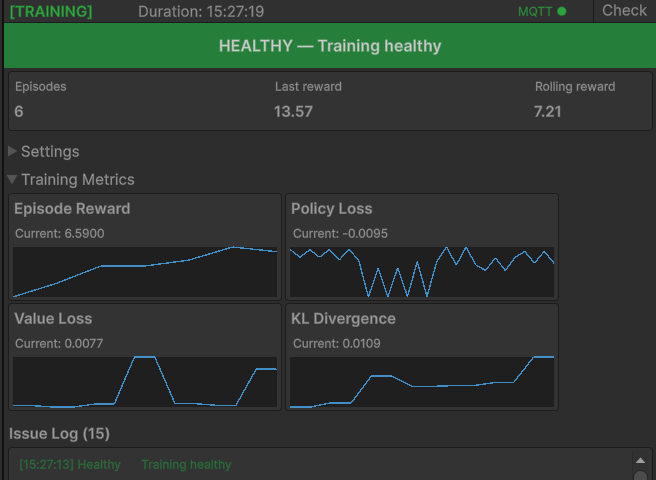
\includegraphics[width=\linewidth]{images/training_graphs.png}
      {\centering\footnotesize\textcolor{upt-gray}{Training convergence graphs (TensorBoard)}\par}

      \vspace{0.4em}
      \begin{itemize}\setlength\itemsep{3pt}
        \item Gymnasium-compliant wrapper — any SB3 algorithm can be substituted
        \item Structured telemetry: \texttt{SHILATE-METRIC} / \texttt{SHILATE-HEALTH} markers parsed live by the Editor
        \item 5-second observation timeout triggers health alert
      \end{itemize}
  \end{columns}
\end{frame}

% ─── SLIDE 6 — Eclipse Leda SDV Integration ──────────────────────────────────
\begin{frame}{Eclipse Leda SDV Integration}
  \begin{columns}[T]
    \column{0.46\textwidth}
      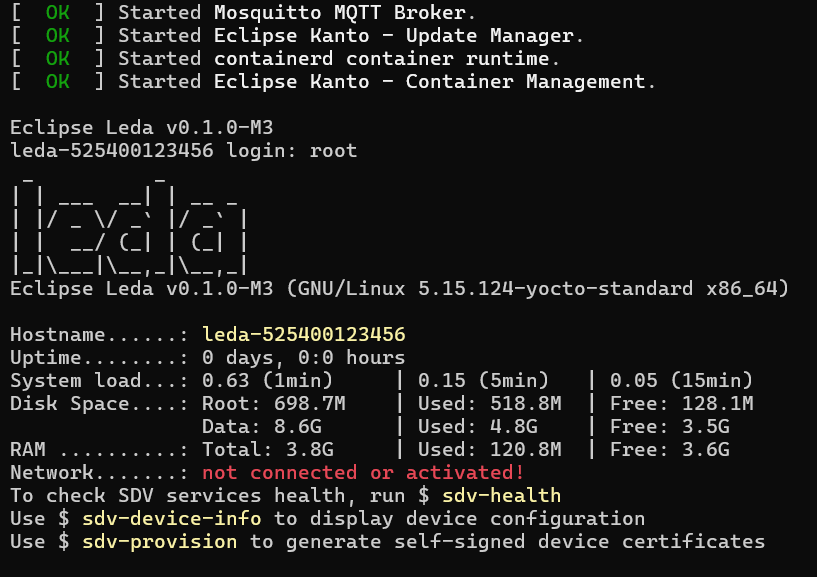
\includegraphics[width=0.92\linewidth]{images/eclipse_leda.png}
      {\centering\footnotesize\textcolor{upt-gray}{Eclipse Leda container stack}\par}

      \vspace{0.4em}
      \small
      \begin{block}{5-Container Docker Compose Stack}
        \begin{enumerate}\setlength\itemsep{2pt}
          \item \textbf{Mosquitto} — MQTT broker
          \item \textbf{Kuksa databroker} — VSS signal store
          \item \textbf{mqtt-kuksa-feeder} — MQTT → VSS bridge
          \item \textbf{Velocitas app} — safety monitor
          \item \textbf{leda-controller} — RL inference engine
        \end{enumerate}
      \end{block}

    \column{0.52\textwidth}
      \textbf{Signal Chain}
      \begin{itemize}\setlength\itemsep{4pt}
        \item \texttt{env0/vehicle/speed} mapped to \texttt{Vehicle.Speed} (COVESA VSS)
        \item Kuksa databroker stores all VSS values
        \item Velocitas app enforces safety limits:
          \begin{itemize}
            \item Overspeed alert if speed $>$ 120~km/h
            \item RPM alert if RPM $>$ 6\,500
          \end{itemize}
      \end{itemize}

      \vspace{0.5em}
      \textbf{Deployment to Raspberry Pi~4}
      \begin{itemize}\setlength\itemsep{4pt}
        \item \texttt{deploy-pi.sh} — ARM64 cross-compile via \texttt{docker buildx}
        \item Transfers images over SSH/SCP, starts stack with \texttt{docker compose up -d}
        \item \alert{Full deploy cycle: $\approx$14 minutes}
      \end{itemize}

      \vspace{0.4em}
      \textbf{Remote Inference} — Training Controller targets the Pi broker; no code changes, policy runs on-device
  \end{columns}
\end{frame}

% ─── SLIDE 7 — Experimental Results ─────────────────────────────────────────
\begin{frame}{Experimental Results}
  \begin{columns}[T]
    \column{0.47\textwidth}
      \textbf{Training Convergence} {\small (3 seeds, mean)}
      \begin{center}
        \small
        \begin{tabular}{lrr}
          \toprule
          Milestone & Timestep & $\sigma$ \\
          \midrule
          First collision-free episode & 12\,400 & $\pm$2\,100 \\
          Half-turn bonus triggered    & 31\,000 & $\pm$3\,800 \\
          \alert{First full lap}       & \alert{48\,500} & $\pm$5\,200 \\
          Rolling mean $\geq 60$       & 76\,000 & $\pm$6\,900 \\
          \bottomrule
        \end{tabular}
      \end{center}

      \vspace{0.5em}
      \textbf{Inference — 50 episodes (local)}
      \begin{center}
        \small
        \begin{tabular}{lr}
          \toprule
          Metric & Value \\
          \midrule
          \alert{Lap completion rate}   & \alert{82\%} \\
          Mean episode reward           & 63.4 \\
          Mean lap duration             & 38.2~s \\
          Mean speed (completed laps)   & 47.6~km/h \\
          Collisions per episode        & 0.6 \\
          \bottomrule
        \end{tabular}
      \end{center}

    \column{0.51\textwidth}
      \textbf{Ablation Study}
      \begin{itemize}\setlength\itemsep{3pt}
        \item Half-turn bonus removed ($c_h=0$): first lap delayed by \alert{$\approx$18\,000 steps}; rolling mean 12 pts lower at 100K
        \item Weaker collision penalty ($c_c=-1$): laps completed but agent drove closer to walls
      \end{itemize}

      \vspace{0.5em}
      \textbf{Health Monitoring — All Failure Modes Detected}
      \begin{itemize}\setlength\itemsep{3pt}
        \item Observation timeout ($>5$~s) → \textit{Critical}
        \item Python crash → non-zero exit code
        \item MQTT disconnect → \textit{Disconnected} within 35~s
      \end{itemize}

      \vspace{0.5em}
      \textbf{Raspberry Pi Remote Inference}
      \begin{center}
        \small
        \begin{tabular}{lr}
          \toprule
          Metric & Value \\
          \midrule
          \alert{Lap completion rate (LAN)} & \alert{74\%} \\
          Additional latency (LAN) & 15–20~ms \\
          Deploy time              & $\approx$14 min \\
          \bottomrule
        \end{tabular}
      \end{center}
  \end{columns}
\end{frame}

% ─── SLIDE 8 — Conclusions ────────────────────────────────────────────────────
\begin{frame}{Conclusions}
  \begin{columns}[T]
    \column{0.60\textwidth}
      \textbf{What was achieved}
      \begin{itemize}\setlength\itemsep{5pt}
        \item \alert{End-to-end RL $\to$ SDV pipeline} — same MQTT/VSS protocol from Unity training to Raspberry Pi~4 hardware
        \item Agent converges within \alert{100\,000 timesteps}; 82\% lap completion in inference
        \item One-click Training Controller with \alert{5-failure-mode health monitoring}
        \item Validated on physical hardware — 74\% remote lap completion over LAN
        \item Curriculum scaling: automatic obstacle density increase with agent skill
        \item Parallel training via Headless Orchestrator (up to 30 environments)
      \end{itemize}

    \column{0.38\textwidth}
      \begin{block}{Future Work}
        \begin{itemize}\setlength\itemsep{4pt}
          \item Domain randomisation for sim-to-real transfer
          \item Safety monitor → active command override (not just alerts)
          \item Multi-agent scenarios and cooperative driving
          \item CAN bus hardware-in-loop testing on real ECUs
        \end{itemize}
      \end{block}

      \vspace{0.8em}
      \centering
      
\includegraphics[width=0.65\linewidth]{images/logo.png}
  \end{columns}

  \vspace{0.8em}
  \begin{center}
    \Large\textbf{Thank you!} \quad
    {\normalsize Questions?}
  \end{center}
\end{frame}

\end{document}
